\documentclass[12pt,letterpaper]{article}

% --- Paquetes Requeridos ---
\usepackage[utf8]{inputenc}
\usepackage[spanish,es-tabla]{babel}
\usepackage[margin=2.5cm]{geometry}
\usepackage{graphicx}
\usepackage{float}
\usepackage{titlesec}
\usepackage{setspace}
\usepackage{hyperref}
\usepackage{booktabs}
\usepackage{caption}
\usepackage{enumitem}
\usepackage{listings}
\usepackage{xcolor}

% --- Configuración de Párrafo ---
\onehalfspacing
\setlength{\parindent}{0pt}
\setlength{\parskip}{1em}

% --- Rutas de búsqueda de imágenes ---
% Permite compilar tanto desde Documentos/Entregables/ como con todas las
% imágenes en una sola carpeta plana.
\graphicspath{{./}{../Evidencia/}{Evidencia/}{imagenes/}}

% --- Configuración de listings ---
\lstset{
    basicstyle=\ttfamily\footnotesize,
    breaklines=true,
    frame=single,
    captionpos=b,
    showstringspaces=false
}

% --- Inicio del Documento ---
\begin{document}

% --- PORTADA ---
\begin{titlepage}
    \centering

    {\Large \textbf{UNIVERSIDAD SANTO TOMÁS}} \\[1cm]

    {\Large \textbf{Sistema colaborativo de robots móviles para asistencia de orientación en entornos interiores con múltiples pisos}} \\[2cm]

    {\large \textbf{Realizado por:}} \\
    {\large Santiago Hernández Ávila} \\
    {\large Jonny Alejandro Mejía León} \\[1cm]

    \begin{figure}[H]
        \centering
        \includegraphics[width=0.6\textwidth]{Logos Uni.png}
        \label{Logo Universidad Santo Tomas y facultad de ingenieria electronica}
    \end{figure}

    \vfill

    {\large \textbf{Informe de Avance --- Semana 24}} \\
    {\large Fase 5: Integración del sistema y realización de pruebas --- El sistema llega al vehículo real: actuación, odometría, mapa y navegación sobre hardware} \\[1.5cm]

    \textbf{Dirigido por:} \\
    Ing. Armando Mateus Rojas, Msc. \\
    Ing. Nestor Ivan Ospina, Msc. \\
    Ing. Oscar Mauricio Gélvez Lizarazo, Msc. \\[1.0cm]

    \vfill

    {\large GED (Grupo de Estudio y Desarrollo en Robótica)} \\
    {\large Facultad de Ingeniería Electrónica} \\
    {\large División de Ingenierías} \\
    {\large Bogotá, septiembre de 2026}
\end{titlepage}

% --- CONTENIDO ---

\section{Introducción}

El presente informe documenta el avance correspondiente a la \textbf{Semana 24} del cronograma de actividades (21 al 27 de septiembre de 2026, con corte el viernes 25), dentro de la \textbf{Fase 5 (Integración del sistema y realización de pruebas)}.

El cronograma reservaba esta semana para la campaña experimental en simulación, que se había adelantado a la Semana 21; lo que quedaba de ella ---consolidar los datos y escribir los resultados--- se cumplió (Sección \ref{sec:objetivos}). \textbf{La semana, en cambio, fue la del vehículo real}: empezó con la decisión de intentar la demostración física y terminó con \textbf{Nav2 navegando el carro de forma autónoma} sobre un mapa que el propio carro había construido.

El acta de decisión fija seis compuertas con fecha. Su estado al cierre de la semana es el siguiente:

\begin{table}[H]
    \centering
    \small
    \caption{Las seis compuertas del acta al cierre de la Semana 24.}
    \label{tab:compuertas}
    \begin{tabular}{@{}p{3.4cm}p{5.6cm}p{5.0cm}@{}}
        \toprule
        \textbf{Compuerta} & \textbf{Qué pide} & \textbf{Estado} \\ \midrule
        G-1 actuación & El vehículo responde a las órdenes de servo & \textbf{Alcanzada}, 22 de septiembre \\ \addlinespace
        G-4 dos en el grafo & Dos vehículos y el coordinador sin colisión de nombres & \textbf{Alcanzada}, 22 de septiembre \\ \addlinespace
        G-2 odometría & Error $\leq$ 10~\% sobre un recorrido medido de $\geq$ 5~m & Medida sobre 3~m; falta la de 5~m con cinta \\ \addlinespace
        G-3 navegación de uno & Punto a punto con Nav2, llegada verificada & Navegó una vez; paró a 0,412~m con tolerancia de 0,25~m \\ \addlinespace
        G-5 protocolo completo & Una misión con relevo sobre los dos vehículos & Pendiente \\ \addlinespace
        G-6 RF-27 & Entre 5 y 10 misiones con el protocolo completo & Pide primero G-5 \\ \bottomrule
    \end{tabular}
\end{table}

G-2 y G-3 tienen fecha: el \textbf{corte C-1 del viernes 2 de octubre}.

\section{Objetivos de la Semana}
\label{sec:objetivos}

El cronograma fija para esta semana el siguiente criterio de cierre:

\begin{quote}
\textit{30 corridas registradas y conjunto de datos versionado en el repositorio.}
\end{quote}

\textbf{Cumplido.} Las 30 corridas se hicieron en la Semana 21, y la consolidación del 21 de septiembre comprobó lo que hace útil a un conjunto de datos: \textbf{que un tercero, con solo el repositorio, llegue de los registros a las cifras publicadas}. El capítulo de resultados se escribió por adelantado el 19 de septiembre.

\textbf{Con una reserva que se abrió el viernes (riesgo R15):} el mapa con que corrió aquella campaña leía como libre su espacio desconocido. No invalida el veredicto por sí solo ---los cuatro fallos fueron de precisión de llegada, no de trazado---, pero queda por decidir si se comprueba sobre las grabaciones conservadas o se declara como limitación.

\section{La decisión: GO pleno, con los criterios de reversión escritos antes}

El 21 de septiembre se resolvió el GO/NO-GO, abierto tres semanas: \textbf{la demostración física se intenta con los dos vehículos reales}. Lo que lo hace defendible no es el veredicto sino sus \textbf{seis compuertas con criterio de fallo y fecha escritos antes de intentarlas}, para que el GO no pueda degradarse en silencio. El mismo día se cerró el riesgo R6 con una fe de erratas del informe de la Semana 15 ---que solo existe como PDF--- en lugar de reescribirlo.

\section{Una sola causa para tres semanas de síntomas}
\label{sec:causa}

El segundo vehículo se había dado por averiado, y \textbf{no lo estaba}. Los nodos del fabricante corren como \texttt{root}, y el middleware de ROS 2 comparte memoria con permisos solo del dueño: una orden lanzada como usuario normal \textbf{descubre los nodos pero no se comunica con ellos, y no da ningún error}. Eso explicaba a la vez listas de nodos vacías, servicios que no respondían y órdenes que no movían nada.

Con el dueño correcto, el 22 de septiembre se alcanzaron dos compuertas. \textbf{G-1, actuación}: dirección a los dos lados y proporcional, tracción en los dos sentidos, y parada en menos de un segundo al soltar la orden. \textbf{G-4, dos en el grafo}: los dos vehículos y el coordinador conviviendo sin colisión de nombres. Y la primera mitad de \textbf{RF-16} sobre hardware: los 22 ficheros del coordinador tienen \textbf{el mismo md5} en el repositorio y en los dos vehículos, y compilan sin un aviso en las dos distribuciones.

\section{Los vehículos se grababan el uno al otro}

El 23 de septiembre se descubrió que, con los dos vehículos encendidos, \textbf{la grabación de uno recoge también el LiDAR del otro}, intercalado, en un archivo que parece sano. Con cuatro confirmaciones independientes, \textbf{los cinco registros de la salida del 28 de agosto quedan retirados}. No hay comprobación en vivo que lo detecte, así que la regla es operativa: \textbf{un solo vehículo encendido}, y la comprobación se hace sobre la grabación ya hecha.

El mismo día, ensayar el guion de campo contra el vehículo encontró \textbf{tres defectos que no daban error}; el peor, que interrumpir una orden remota dejaba el grabador huérfano y grabando.

\section{La escalera de Nav2, peldaño a peldaño sobre el vehículo}
\label{sec:escalera}

El 24 de septiembre la cadena de navegación se subió \textbf{por peldaños}, comprobando cada uno antes del siguiente.

\subsection{Peldaños 1 a 3: la odometría mide}

La transformada del vehículo quedó versionada, y \texttt{rf2o} publica la odometría. Sobre \texttt{amss-jgm9}, empujando a mano tres recorridos de 3,00~m medidos con flexómetro:

\begin{table}[H]
    \centering
    \small
    \caption{Odometría contra cinta sobre 3,00~m.}
    \label{tab:odometria}
    \begin{tabular}{@{}cc@{}}
        \toprule
        \textbf{Pasada} & \textbf{Odometría $\div$ cinta} \\ \midrule
        1 & 0,963 \\
        2 & 1,019 \\
        3 & 0,966 \\ \bottomrule
    \end{tabular}
\end{table}

Media \textbf{0,982}, $\sigma$ 0,032: \textbf{las tres dentro del $\pm$10~\%}. \textbf{No es todavía G-2}: son 3~m, G-2 pide 5, y el sitio tenía estructura por los cuatro lados.

\subsection{Peldaños 4 y 5: el mapa sobre el vehículo}

El SLAM corrió a bordo por primera vez. En un cuarto de 1,60 $\times$ 0,76~m medidos con cinta, la sala salió de 1,50 $\times$ 0,80~m y de 1,60 $\times$ 0,95~m en dos corridas; y un extintor puesto como obstáculo apareció como una mancha aislada de 0,25 $\times$ 0,15~m.

\subsection{Mapear conduciendo}

El vehículo se condujo solo por el pasillo del piso 2 midiendo contra su odometría ---6,093~m y 6,032~m con 6,00 pedidos---, con una deriva en reposo de 1 a 25~mm, y construyó el mapa de la Figura \ref{fig:mapa}.

\begin{figure}[H]
    \centering
    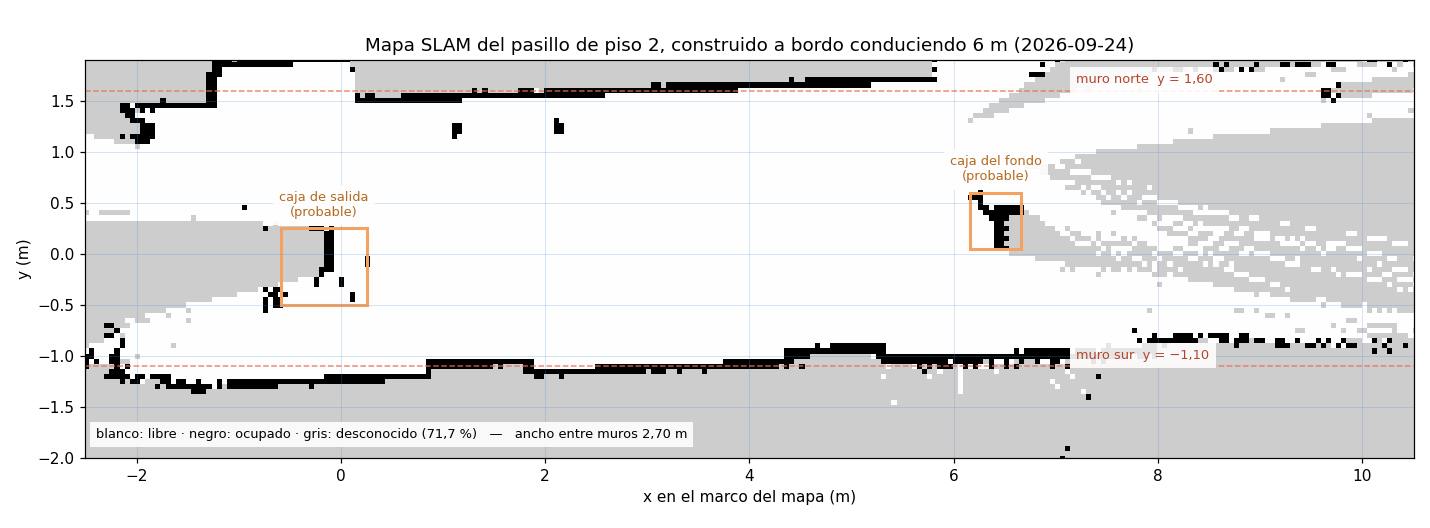
\includegraphics[width=\textwidth]{S24_mapa_pasillo6m_HARDWARE.png}
    \caption{Mapa del pasillo del piso 2 construido a bordo conduciendo 6~m: 447 $\times$ 108 celdas de 5~cm, pasillo de 2,70~m entre muros, y dos objetos aislados que son, casi con seguridad, las cajas que acotaban el tramo.}
    \label{fig:mapa}
\end{figure}

\subsection{Peldaños 6 y 7: Nav2 navega el carro}

Esa misma noche se cargó ese mapa y \textbf{Nav2 llevó el vehículo de forma autónoma} (Figura \ref{fig:navegacion}).

\begin{figure}[H]
    \centering
    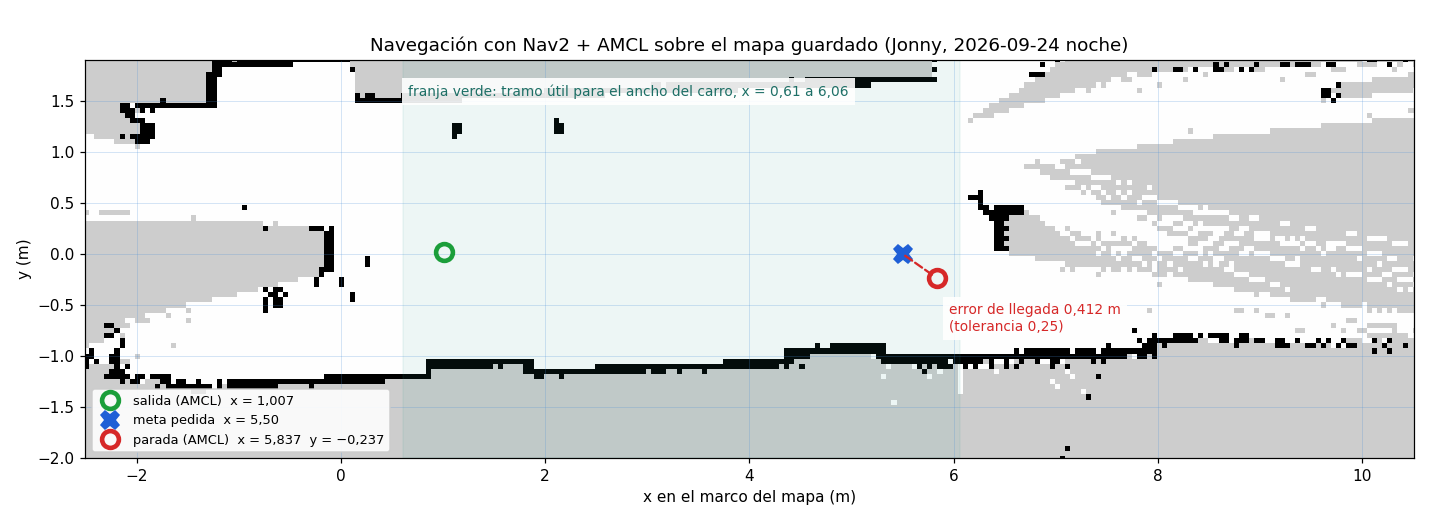
\includegraphics[width=\textwidth]{S24_nav2_navegacion_mapa_guardado.png}
    \caption{Navegación con Nav2 y AMCL sobre el mapa guardado: de x = 1,007 hacia una meta en x = 5,50, avance de 4,837~m y parada a 0,412~m de la meta.}
    \label{fig:navegacion}
\end{figure}

Que fue navegación y no un empujón lo dicen tres cosas de la grabación: el plan \textbf{se fue consumiendo} (de 59 a 7 poses), \textbf{la dirección trabajó} ---corrigiendo el rumbo cuando el carro se desviaba--- y las órdenes salieron del planificador. \textbf{La precisión de llegada no}: 0,412~m contra una tolerancia de 0,25. La causa está medida: por debajo de 0,40~m/s el vehículo no se mueve, así que se aproxima a la meta sin poder frenar antes, y la sobrepasa.

\section{Las compuertas, montadas; el bloqueo del sistema real, diseñado}
\label{sec:campana}

El 25 de septiembre quedó lista la sesión que convierte esa navegación en G-2 y G-3, en \texttt{GUIA\_CAMPANA\_NAV2\_HARDWARE.md}, escrita para que la ejecute cualquiera que descargue el repositorio (Figura \ref{fig:campana}).

\begin{figure}[H]
    \centering
    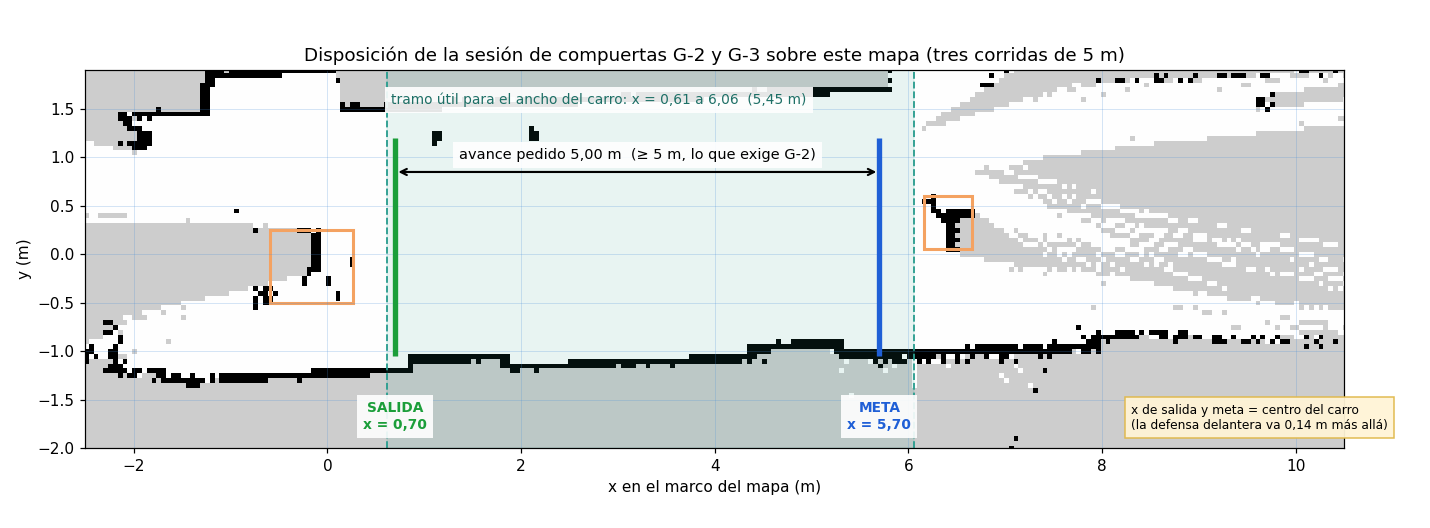
\includegraphics[width=\textwidth]{S24_campana_disposicion_pasillo6m.png}
    \caption{Disposición de la sesión de compuertas sobre el mapa. El tramo útil para el ancho del carro mide 5,45~m, así que caben corridas de 5~m ---lo que pide G-2--- sin volver a mapear.}
    \label{fig:campana}
\end{figure}

\begin{itemize}[leftmargin=*]
    \item \textbf{Tres corridas de 5~m con cinta cierran G-2 y dan G-3.} No cuentan para RF-27, que pide el protocolo completo sobre los dos carros.
    \item \textbf{El bloqueo del sistema real, diseñado.} Con los dos carros encendidos, una orden mueve los dos y cada odometría recibe el láser del otro, porque los tópicos de fábrica no llevan espacio de nombres. La solución ---una partición DDS por vehículo para esos tópicos, sin tocar el software de AWS--- pasó \textbf{9 de 9} en el portátil y se confirma en los carros el lunes 28 (\texttt{DISENO\_AISLAMIENTO\_DOS\_CARROS.md}).
    \item La herramienta que ejecuta cada corrida se \textbf{ensayó contra Nav2 en simulación} con los vehículos apagados. El ensayo encontró que la pose de AMCL, al parar, puede ir \textbf{hasta 25~cm atrasada}; forzando su corrección, AMCL y la odometría quedan a \textbf{1,7~cm}.
    \item En paralelo se escribió \texttt{GUION\_NAVEGACION\_USTA.md}, la vía hermana: navegar el edificio sobre el mapa del modelo de Gazebo, \textbf{validando antes el modelo contra el edificio con flexómetro} ($\leq$ 2~\%). Las dos comparten el arranque, \texttt{nav2\_mapa\_guardado.sh}.
    \item Ver la corrida después, en RViz, funciona. \textbf{Verla en vivo desde el portátil no}: las dos distribuciones de ROS se descubren pero no intercambian datos, y está medido.
\end{itemize}

\section{Lo que la semana corrigió de sí misma}

Cinco conclusiones de esta misma semana resultaron falsas, y se publican corregidas en vez de borrarse:

\begin{enumerate}[leftmargin=*]
    \item \textbf{La ``avería'' del segundo vehículo} (21 de septiembre) no existía: era la regla del dueño de la Sección \ref{sec:causa}.
    \item \textbf{Que el LiDAR se podía leer sin privilegios} (24 de septiembre, mañana) se refutó esa misma tarde con cero barridos en 20~s.
    \item \textbf{Que \texttt{amss-jgm9} no tenía Nav2 ni rf2o, y que Nav2 no podía navegar por cuatro defectos de configuración} (24 de septiembre, noche): falso las dos veces. El vehículo estaba nivelado ese día, y los defectos eran de un fichero que el vehículo no carga. Nav2 navegó esa misma noche.
    \item \textbf{Que el carro ``avanzó 5~m''} (25 de septiembre): es la distancia entre las cajas y la impresión de que llegó cerca, no una medida.
    \item \textbf{Que las corridas de un solo carro contaban para RF-27} (25 de septiembre): RF-27 pide el protocolo completo, con los dos carros y el relevo entre pisos.
\end{enumerate}

\section{Aporte de la semana a los objetivos específicos}
\label{sec:aporte}

\subsection{Relación entre actividades y objetivos}

\begin{table}[H]
    \centering
    \small
    \caption{Trazabilidad entre las actividades ejecutadas y los objetivos específicos.}
    \label{tab:trazabilidad}
    \begin{tabular}{@{}p{4.6cm}cp{7.2cm}@{}}
        \toprule
        \textbf{Actividad} & \textbf{Objetivo} & \textbf{Contribución} \\ \midrule
        Acta GO/NO-GO & OE2, OE4 & Fija qué se intenta y cuándo se desiste, antes de intentarlo \\ \addlinespace
        Causa raíz de la comunicación con el vehículo & OE2 & Explica tres semanas de síntomas y desbloquea todo lo demás \\ \addlinespace
        G-1 y G-4 & OE2 & Actuación y dos vehículos en el mismo grafo, verificados \\ \addlinespace
        Odometría medida sobre 3~m & OE2 & Primera evidencia física de RF-13 \\ \addlinespace
        SLAM y Nav2 sobre el vehículo & OE2, OE4 & La navegación autónoma física existe \\ \addlinespace
        Sesión de compuertas y diseño del aislamiento & OE2, OE4 & Deja G-2 y G-3 medibles antes del corte, y desbloquea el sistema real \\ \addlinespace
        Consolidación de datos & OE4 & Criterio de cierre de la semana \\ \bottomrule
    \end{tabular}
\end{table}

\subsection{Estado de los objetivos específicos}

\begin{table}[H]
    \centering
    \small
    \caption{Avance por objetivo específico al cierre de la Semana 24.}
    \label{tab:objetivos}
    \begin{tabular}{@{}cp{2.6cm}p{4.6cm}p{4.4cm}@{}}
        \toprule
        \textbf{ID} & \textbf{Avance} & \textbf{Cubierto esta semana} & \textbf{Componente que lo mantiene detenido} \\ \midrule
        OE1 & 100~\% & --- & --- \\ \addlinespace
        OE2 & \textbf{65~\%}, sin cambio & G-1, G-4, odometría, SLAM y Nav2 sobre el vehículo & Ninguno de sus cinco requisitos parciales cerró todavía \\ \addlinespace
        OE3 & 100~\% & --- & --- \\ \addlinespace
        OE4 & \textbf{85~\%}, sin cambio & Datos consolidados & RF-27, que pide el sistema completo; y la decisión sobre R15 \\ \bottomrule
    \end{tabular}
\end{table}

El avance agregado sin ponderar sigue en \textbf{87,5~\%}, frente a un \textbf{75,0~\%} del calendario (semana 24 de 32). \textbf{Veintinueve de treinta y seis requisitos verificados}, los mismos que la semana anterior.

\textbf{Por qué el objetivo 2 no sube en la semana en que más avanzó.} El porcentaje se mueve cuando un requisito cierra, y ninguno de los cinco parciales del objetivo 2 cerró: cada uno tiene ahora evidencia sobre el vehículo, pero les falta la medida de 5~m, el espacio de nombres o la segunda mitad de su criterio. Subirlo por la sensación de avance sería exactamente lo que el tablero existe para impedir. \textbf{Lo que sí cambió es el riesgo}: la navegación autónoma física ya no es una pregunta abierta.

\section{Estado del cronograma y trabajo previsto}
\label{sec:cronograma}

\subsection{Cumplimiento del criterio de cierre}

\begin{table}[H]
    \centering
    \small
    \caption{Criterio de cierre de la Semana 24 y su evidencia.}
    \label{tab:cierre}
    \begin{tabular}{@{}p{5.6cm}cp{6.0cm}@{}}
        \toprule
        \textbf{Exigencia del criterio} & \textbf{Estado} & \textbf{Evidencia} \\ \midrule
        30 corridas registradas & Cumplido & Semana 21; 30 registros validados \\ \addlinespace
        Conjunto de datos versionado & Cumplido & Consolidación del 21 de septiembre: regenera sus propias métricas \\ \bottomrule
    \end{tabular}
\end{table}

\subsection{Lo planificado frente a lo hecho}

Las tres actividades planificadas se cumplieron: consolidar los datos, escribir el capítulo de resultados ---adelantado a la Semana 23--- y emitir el informe de la Semana 23. \textbf{Todo el trabajo sobre el vehículo real no estaba planificado para esta semana} y se declara como tal: el cronograma lo situaba en la Semana 25, y lo que se hizo aquí es la preparación que lo hace posible.

\subsection{Trabajo previsto para la Semana 25}

Con el plan día a día en \texttt{PLAN\_S25.md}: la sesión de compuertas G-2 y G-3 antes del corte C-1 del \textbf{viernes 2 de octubre}; aislar los dos carros y montar la pila con espacio de nombres; validar con cinta el modelo del edificio y medir la red entre pisos; y pedir por escrito a los directores el sitio de la etapa 3, el N de RF-27 y la tolerancia de llegada. \textbf{El sistema real ---G-5--- va en la Semana 26 y la campaña de RF-27 en la 27}, con cierre de datos el 16 de octubre.

\section{Conclusiones de la Semana}

\begin{enumerate}[leftmargin=*]
    \item \textbf{El sistema llegó al vehículo real.} En cinco días se pasó de decidir intentarlo a que Nav2 navegara el carro de forma autónoma sobre un mapa construido por el propio carro.
    \item \textbf{Una sola causa explicaba tres semanas de síntomas}, y encontrarla desbloqueó dos compuertas el mismo día.
    \item \textbf{La odometría del vehículo mide}: tres de tres dentro del $\pm$10~\% sobre 3~m. Falta la medida de 5~m con cinta, que es G-2.
    \item \textbf{La navegación funciona y la precisión de llegada no}, con el mecanismo medido. La tolerancia es decisión de los directores y tiene que tomarse antes de la campaña.
    \item \textbf{La sesión que cierra G-2 y G-3 está montada, ensayada en simulación y documentada}, y el bloqueo que impide el sistema real ---los dos carros pisándose--- tiene un diseño probado en el portátil.
    \item \textbf{Cinco conclusiones de la semana se corrigieron dentro de la misma semana}, y se publican corregidas.
\end{enumerate}

\section{Anexos}

Las cifras de este informe proceden de los registros y documentos de evidencia versionados en el repositorio del proyecto. Existe una versión en Markdown de este mismo informe, \texttt{Entregable\_semana\_24.md}, legible directamente en el repositorio.

\begin{thebibliography}{99}

\bibitem{acta}
S. Hernández Ávila y J. A. Mejía León,
``Acta de decisión GO/NO-GO de la demostración física,''
Repositorio del proyecto, \texttt{Documentos/ACTA\_GO\_NOGO.md}, septiembre de 2026.

\bibitem{g1}
S. Hernández Ávila,
``Sonda de actuación sobre \texttt{amss-ez9n}: la compuerta G-1,''
Repositorio del proyecto, \texttt{Documentos/Evidencia/S24\_sonda\_actuacion\_amss\_ez9n.md}, septiembre de 2026.

\bibitem{g4}
S. Hernández Ávila,
``Compuerta G-4: dos vehículos en el mismo grafo,''
Repositorio del proyecto, \texttt{Documentos/Evidencia/S24\_compuerta\_G4\_dos\_en\_el\_grafo.md}, septiembre de 2026.

\bibitem{rf16}
S. Hernández Ávila,
``RF-16: compilación del coordinador sobre hardware,''
Repositorio del proyecto, \texttt{Documentos/Evidencia/S24\_RF16\_compilacion\_jazzy\_hardware.md}, septiembre de 2026.

\bibitem{odometria}
J. A. Mejía León,
``Peldaño 2: la odometría del vehículo medida contra flexómetro,''
Repositorio del proyecto, \texttt{Documentos/Evidencia/S24\_peldano2\_odometria\_hardware.md}, septiembre de 2026.

\bibitem{mapeo}
S. Hernández Ávila,
``El vehículo se conduce solo seis metros y construye el mapa,''
Repositorio del proyecto, \texttt{Documentos/Evidencia/S24\_mapeo\_6m\_hardware.md}, septiembre de 2026.

\bibitem{nav2}
J. A. Mejía León,
``Peldaños 6 y 7: Nav2 navega el vehículo sobre un mapa guardado,''
Repositorio del proyecto, \texttt{Documentos/Evidencia/S24\_nav2\_navegacion\_mapa\_guardado.md}, septiembre de 2026.

\bibitem{consolidacion}
S. Hernández Ávila,
``El conjunto de datos de OE4, consolidado,''
Repositorio del proyecto, \texttt{Documentos/Evidencia/S24\_consolidacion\_datos\_oe4.md}, septiembre de 2026.

\bibitem{campana}
S. Hernández Ávila y J. A. Mejía León,
``Guía de la campaña de navegación con Nav2 sobre el vehículo real,''
Repositorio del proyecto, \texttt{Documentos/GUIA\_CAMPANA\_NAV2\_HARDWARE.md}, septiembre de 2026.

\end{thebibliography}

\end{document}
